\documentclass[12pt]{article}
\usepackage[utf8]{inputenc}
\usepackage[margin=2cm]{geometry}
\usepackage{fullpage,enumitem,amssymb,amsmath,xcolor,cancel,gensymb,hyperref,graphicx}
\usepackage{indentfirst}
\usepackage{lipsum}
\usepackage{pgf,tikz}
\graphicspath{ {./images/} }
\setlength{\parskip}{1em}
\usepackage{listings}
\usepackage{xcolor}
\definecolor{codegreen}{rgb}{0,0.6,0}
\definecolor{codegray}{rgb}{0.5,0.5,0.5}
\definecolor{codepurple}{rgb}{0.58,0,0.82}
\definecolor{backcolour}{rgb}{0.95,0.95,0.92}
\usepackage[english]{babel}
\usepackage{amsthm}
\newtheorem*{theorem}{Theorem}

\lstdefinestyle{mystyle}{
    backgroundcolor=\color{backcolour},   
    commentstyle=\color{codegreen},
    keywordstyle=\color{magenta},
    numberstyle=\tiny\color{codegray},
    stringstyle=\color{codepurple},
    basicstyle=\ttfamily\footnotesize,
    breakatwhitespace=false,         
    breaklines=true,                 
    captionpos=b,                    
    keepspaces=true,                 
    numbers=left,                    
    numbersep=5pt,                  
    showspaces=false,                
    showstringspaces=false,
    showtabs=false,                  
    tabsize=2
}

\lstset{style=mystyle}

%\begin{align*}…\end{align*} if you want to fit an equation. 
%FOR PICTURES: include graphicsx 
%\includegraphics[scale=x]{name}
%double space and write caption in the center classshe 

\hypersetup{
colorlinks=true,
linkcolor=black
}

\begin{document}

\begin{titlepage}
\begin{center}

    \vspace*{4cm}
    {\LARGE{\textbf{The Analytical Results of the Oscillatory Behavior in the Willson-Cowan Neuronal Model }}\par}

    \vspace{2cm}
    {\large Applied Project Math 303}

    \vspace{2cm}
    {\large
        Chenjun Ji\\
        Sean Guo 
    \par}
    
    \vspace{1cm}
    {\large
    2020/10/20
    \par}

\end{center}
\end{titlepage}

\tableofcontents

\section{ Introduction}

It is known that the information of the features of objects are processed in different cortical areas. However, it is still an open question that how the different features of an object bond together to form a coherent image (Monteiro, Bussab \& Chaui Berlinck, 2002). Von der Malsburg and other authors (von der Malsburg \& Buhmann, 1992) have proposed that these features are linked through temporal correlations of neuronal activities. In other words, the feature is represented by a synchronized oscillation of a neuronal group. Meanwhile, theories and observations have suggested that the oscillatory activity of cortex may be related to the processing of sensations and cognitive functions (e.g., Engel et al., 1992b; Basar et al., 1999).

Based on these facts and hypotheses, we raise our main question that under which conditions the oscillatory behavior of the neural response may appear. The activity of a cortical column is Mathematically described through the model developed by Wilson \& Cowan (1972). The model uses two variables to describe two populations of excitatory or inhibitory cells respectively. In our final project we would use the simplified the model (Monteiro, Bussab \& Chaui Berlinck, 2002) and try to explore the dynamics of the modified system of differential equations. Since the oscillatory behavior may correspond to a limit cycle on the phase plane, we would focus on the occurrence of limit cycles.
First, we look specifically at a particular case when columns do not receive any stimulations and we want to learn the behavior of this system. In this case, we would fix other parameters and only change the variable representing the strength of the self-excitatory connection to see under which condition the limit cycles would appear. We do some analysis on the stability of equilibria and use Mathematical and Python simulation to help verify our analysis. Then, we would make two attempts to see the more general cases when the amount of external stimulation is not equal to zero. In this case, we combine the Mathematical analysis with visualizations to figure out the reasons of occurrence and disappearance of the limit cycles.




\section{ Literature Review}

The Wilson–Cowan model developed in 1972 emphasizes not the individual cell but rather the properties of populations (Wilson \& Cowan, 1972). Wilson and Cowan explain the reasons for this emphasis in the way that: The sensory information is introduced in the form of largescale spatiotemporal activity and pattern recognition is in some sense a global process. Meanwhile, local interactions can be random, but that this local randomness may give rise to quite precise long-range interactions (Wilson \& Cowan, 1972). Thus, it is appropriate to look at the dynamics of neural populations rather than individual cells. In our project, we assume that the basic functional unit is a cortical column instead of a single neuron.

Another crucial assumption of the Wilson–Cowan model is that “all nervous
processes of any complexity are dependent upon the interaction of excitatory and
inhibitory cells” (Wilson \& Cowan, 1972). The failure of considering inhibition led Ashby et al. (1962) to conclude the paradox of dynamical stability of the brain and Griffith (1963) dissolved the paradox by the introduction of inhibition. Thus, it is essential to take both excitatory and inhibitory cells into consideration. And we use two variables separately to describe each population.
In the Wilson–Cowan model (Wilson \& Cowan, 1972) the interaction of excitatory and inhibitory populations is described through a sigmoidal function, which is usually chosen as the hyperbolic tangent or the logistic curve. Both choices make difficult theoretical analyses. A main problem concerning analytical approaches to Wilson–Cowan model rests on the difficulty in finding the conditions for the existence of limit cycle. In 2002, Monteiro, Bussab and Chaui Berlinck bypassed the difficulty by choosing another sigmoidal function and modified the original model (Monteiro, Bussab \& Chaui Berlinck, 2002). In this project, we would use the same modified model derived by them.



\section{ Methods and Results}
\subsection{Model}
  In the study of Monteiro.et.al(2002) ,the model proposed by Wilson and Cowan(1972) in their study converted into
  
  \begin{equation}
    \begin{matrix}
      \frac{d(x)t}{dt}=-ax(t)+(1-r_xx(t))S(wx(t)-by(t)+I(t))
      \\
      \frac{d(y)t}{dt}=-dy(t)+(1-r_yy(t))S(cx(t)-ey(t)+J(t))
      \end{matrix}
  \end{equation}
  \indent Here $x(t)$ and $y(t)$ are respectively $E$ and $I$ in the original model, which represents respectively the "proportion of excitatory or inhibitory cells firing per unit time at instant $t$" (Wilson\&Cowan, 1972, p. 3). $a$ and $d$ represent the natural decay factor, which is taken as the constant $1$ in the original model. $w$ and $e$ respectively represent the excitatory or inhibitory stimulation the cell groups produced to themselves. $b$ and $c$ represent the inhitaory or excitatory stimulation produced between cell groups. $I$ and $J$ are the external stimulations. Relationships between these parameters can be illustated by Graph 1. $S$ corresponds to the response function, which gives the proportion of cells responding to certain levels of stimulation. $S$ is defined as
  \begin{equation}
    S(\theta')=\int_0^{\theta'}D(\theta)d\theta
  \end{equation}

  where $\theta'$ is certain simulation level, $D(\theta)$ is a distribution function of response thresholds within certain cell populations, and $\theta$ represents the stimulation levels. Given the randomness in $D(\theta)$, as Wilson and Cowan(1972) argues, "No particular significance is to be attached to the choice of $S$". Therefore, any sigmoid function can fit in as long as it has the following properties:
  \begin{itemize}
    \item $S(\theta')$ is monotonically increasing.
    \item When $\theta'\to\infty$, $S(\theta')\to C_1$; when $\theta'\to -\infty$, $S(\theta') \to C_2$, where $C_1$ and $C_2$ are real constants. 
    \item $S(\theta')$ has and only has one inflection point.
  \end{itemize}
  Therefore, here we choose the sigmoidal function:
  \begin{equation}
    S(\theta')=\frac{\theta'}{\sqrt{\theta'^2+1}}
  \end{equation}
  Moreover, Wang(1995) proposed that $e$ which is the inhibitary stimulation produced by the inhibitary cells to themselves, does not change the behavior of the model. Therefore, in our project we choose $e=0$. 
\begin{center}
    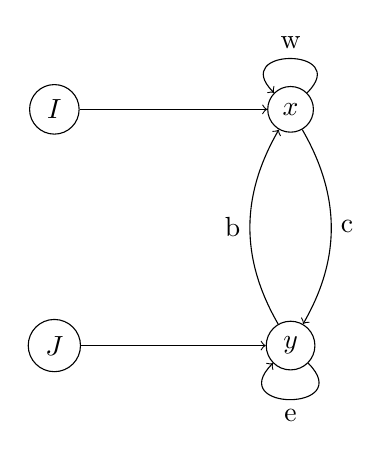
\begin{tikzpicture}[node distance={30mm},main/.style = {draw,circle}]
      \node[main] (1) {$I$};
      \node[main] (2) [below of=1] {$J$};
      \node[main] (3) [right of=1] {$x$};
      \node[main] (4) [below of=3] {$y$};
      \draw[->] (1) -- (3);
      \draw[->] (2) -- (4);
      \draw[->] (3) to[out=-60,in=60,looseness=1] node[midway,right,pos=0.5]{c}(4);
      \draw[->] (4) to[out=120,in=-120,looseness=1] node[midway,left,pos=0.5]{b}(3);
      \draw[->] (3) to[out=45,in=135,looseness=5] node[midway,above,pos=0.5]{w}(3);
      \draw[->] (4) to[out=-45,in=-135,looseness=5] node[midway,below,pos=0.5]{e}(4);
    \end{tikzpicture}
    \\
    \footnotesize{Graph 1. The relationship between parameters}
\end{center}

\indent The model in equation (1) will then be:
\begin{equation}
  \begin{matrix}
    \frac{d(x)t}{dt}=f(x,y)=-ax+\frac{wx-by+I}{\sqrt{(wx-by+I)^2+1}}
    \\
    \frac{d(y)t}{dt}=g(x,y)=-dy+\frac{cx+J}{\sqrt{(cx+J)^2+1}}
    \end{matrix}
\end{equation}

We will use equation (4) in following analyses.

\subsection{Analysis}

\indent To study the state of limit cycle in this planar system, we first look into the state of equilibria, which can be decided by the intersections of $x$-nullclines and $y$-nullclines, where $f(x,y)=0$ and $g(x,y)=0$. As an example, graph 2 illustrates one state of the nullclines. 

\begin{center}
  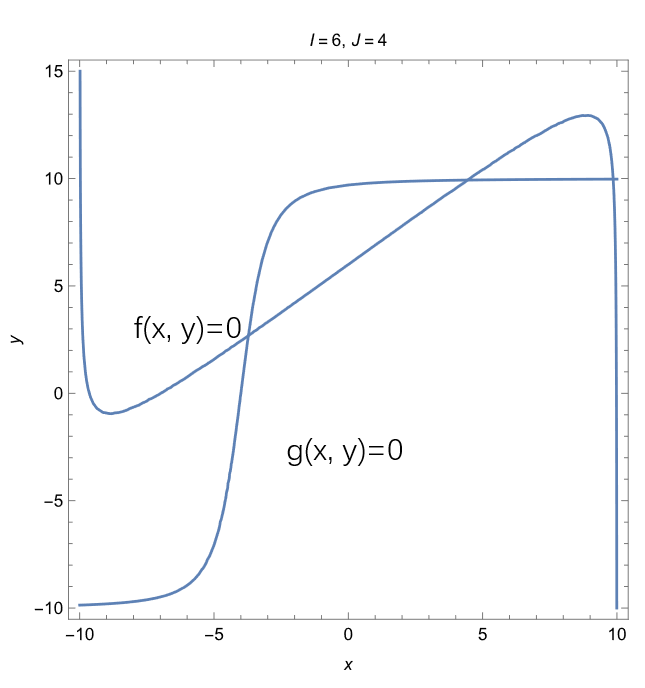
\includegraphics[scale=0.4]{ Nullclines.png} 
  \\
  \footnotesize{Graph 2. Nullclines of the system at $a=0.1,b=1,c=1,d=0.1,w=1,I=6,J=4$, generated by Mathematica.}
\end{center}

\indent The nullclines can be described by curves:

\begin{equation}
  \begin{matrix}
    f(x,y)=0\to y_f(x)=\frac{1}{b}(wx+I-\frac{ax}{\sqrt{1-(ax)^2}}).
    \\
    g(x,y)=0\to y_g(x)=\frac{1}{d}(\frac{cx+J}{\sqrt{1+(cx+J)^2}})
  \end{matrix}
\end{equation}

\indent For $y_f(x)$,it has a local maximum at $x_1$ and a local minimum at $x_2=-x_1$. When $x\to -\frac{1}{a}$, $y_f(x)\to+\infty$, and when $x\to \infty,y_f(x)\to -\infty$.
\newline
\indent For $y_g(x)$, $y_g(x)\to \frac{1}{d}$ when $x\to +\infty$, and $y_g(x)\to-\frac{1}{d}$ when $x\to-\infty$, and $y_g(0)=\frac{J}{(d\sqrt{1+J^2})}$.
\newline
\indent The stability of the equilibrium can be decided by the Jacobian matrix of the system, which is
\begin{equation}
  DF(\mathbf{x})=
  \left[
    \begin{matrix}
      -a+\frac{w}{\sqrt{1+(6+wx-y)^2}}-\frac{w(6+wx-y)^2}{(1+(6+wx-y)^2)^{\frac{3}{2}}}&-\frac{1}{\sqrt{1+(6+wx-y)^2}}+\frac{(6+wx-y)^2}{(1+(6+wx-y)^2)^{\frac{3}{2}}}
      \\
      -\frac{c(4+cx)^2}{(1+(4+cx)^2)^{\frac{3}{2}}}+\frac{c}{\sqrt{1+(4+cx)^2}}&-d      
    \end{matrix}
  \right]
\end{equation}
where the trace $T$ and determinant $D$ are given by
\begin{equation}
  \begin{matrix}
    T=\alpha w -a-d
    \\
    \Delta= ad+bc\alpha \beta-\alpha dw
  \end{matrix}
\end{equation}
\indent Here $\alpha =(1-(ax^{*})^{2})^{\frac{3}{2}}$ and $\beta =(1+(cx^*+J)^2)^{-\frac{3}{2}}$, and $x^*$ is the $x$ coordinate of the equilibrium. 
\newline
\indent Hopf bifurcation is a strong indication of the existence of a limit cycle. Therefore, we need to pay special attention to the conditions for Hopf bifurcation to happen. A key condition for Hopf bifurcation to happen is $T=0$ and $\Delta>0$.When $T$ changes from negative values to positive values, an asymptotically stable limit cycle appears and $x(t)$, $y(t)$ present oscillatory behavior. 
\subsection{A Particular Case}
\indent In this project we focus on the case where there is no external stimulation and see if there can be any oscillatory behavior. Therefore, in this particular case  we choose $I=0$ and $J=0$. 

In this case, $w$ is the most important parameter, as it represents the strength of the self-excitatory connection and is the only source of stimulation in this case. Therefore, in this case we focus on the change of $w$ and its influence on the existence of a limit cycle. 

For the convenience of analysis, $a$, the natural decay factor for the excitatory cells is also taken to be zero. The model then is:

\begin{equation}
  \begin{matrix}
  \frac{dx}{xt}=f(x,y)=\frac{wx-by}{\sqrt{(wx-by)^2+1}}\\
  \frac{dy}{dt}=g(x,y)=-dy+\frac{cx}{cx^2+1}
  \end{matrix}
\end{equation}
\indent By solving $\left\{\begin{matrix} f(x,y)=0
\\g(x,y)=0\end{matrix}\right.$, the coordinates of the equilibria  are:
\begin{align*} 
  &x_a^*=0,y_a^*=0,\\
  &x_b^*=\frac{1}{c}\sqrt{\gamma^2-1},y_b^*=\frac{wx_b^*}{b}\\
  &x_c^*=-x_b^*,y_c^*=-y_b^*
  \end{align*}

\indent Define $\gamma\equiv \frac{bc}{dw}$. 

\indent For the equilibrium $(0,0)$, in this case the trace $T=w-d$, $\Delta=g(x,y)=-dy+\frac{cx}{cx^2+1}$. $T<0$ when $w<d$, $T>0$ when $w>d$, $T=0$ when $w=0$; $\Delta>0$ when $\gamma>1$, $\Delta=0$ when $\gamma=1$, $\Delta<0$ when $\gamma<1$. According to Graph 3, the stability states of this equilibrium can be separated into three cases: 
\begin{itemize}
  \item $w<d$ ($T<0$), $\gamma>1$($\Delta>0$), stable (node/spiral)
  \item $w>d$ ($T>0$), $\gamma>1$($\Delta>0$), unstable (node/spiral)
  \item $\gamma<1$($\Delta<0$), saddle
\end{itemize}

\indent For other two equilibria, when $\gamma<1$, they do not exist; when $\gamma>1$, $\Delta<0$, they are saddle points. Therefore, the stability states of these two equilibria can be separated into two cases. 
\begin{itemize}
  \item $\gamma<1$, no existence
  \item $\gamma>1$, saddle
\end{itemize}
\begin{center}
  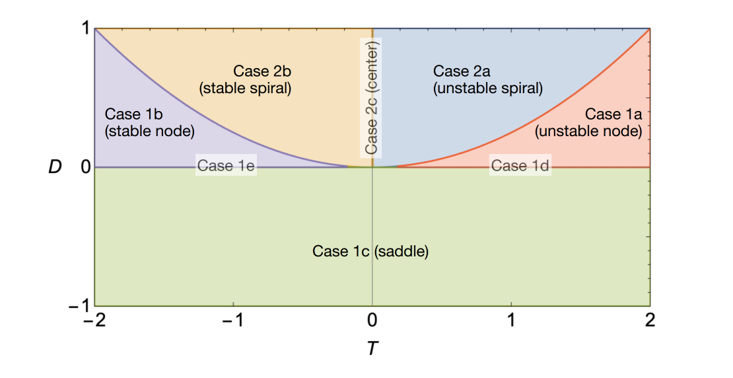
\includegraphics[scale=0.5]{ StabilityExplanation.png}
  \\
  \footnotesize{Graph 3. The $T,D$ plane and the regions of stability.}
\end{center}

  Taken together, there are three cases:
  \begin{itemize}
    \item $\gamma<1$, the other two equilibria do not exist and $(0,0)$ is a saddle point.
    \item $\gamma>1$, $w<d$, the other two equilibria are saddle points and $(0,0)$ is stable node/spiral.
    \item $\gamma<1$, $w>d$, the other two equilibria are saddle points and $(0,0)$ is unstable node/spiral.
  \end{itemize}


  This can be illustrated in the following example. When we take $b=1,c=1,d=0.5$, and change the value of $w$, we can see the change in equilibria. In this example, there are accordingly three cases of stability:
  \begin{itemize}
    \item $w<0.5$ ($w<d,\gamma>1$), the other two equilibria are saddle points and $(0,0)$ is a stable spiral/node.
    \item $w>2$ ($w>d,\gamma<1$), the other two equilibria do not exist and $(0,0)$ is a saddle point.
    \item $0.5<w<2$ ($w>d,\gamma>1$), the other tow equilibria are saddle points and $(0,0)$ is an unstable spiral/node. 
  \end{itemize}

  Simulate this example with Listing 1 and we get results in Graph 4, which agrees with our theories above. In the graph, the solid blue lines are nullclines of the system and their intersections represent the equilibria. The red solid line is the trajectory starting from a point near the origin and tracing through $t=0$ to $t=100$, where $t$ is the unit time.

\begin{center}
  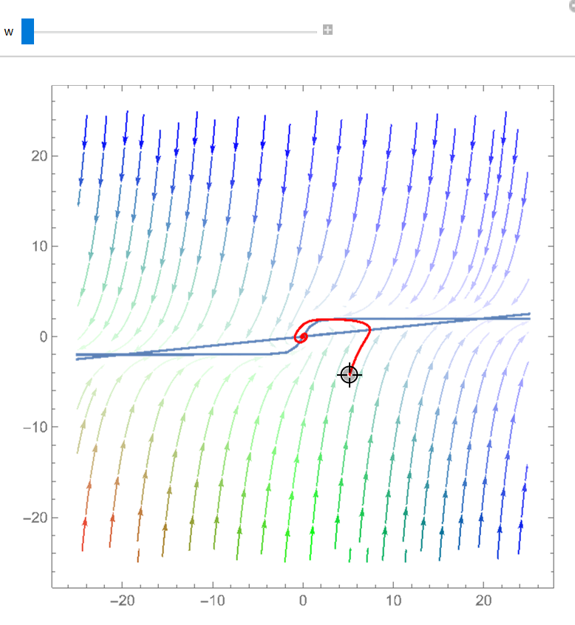
\includegraphics[scale=0.3]{ StabilitySketch00.png}
  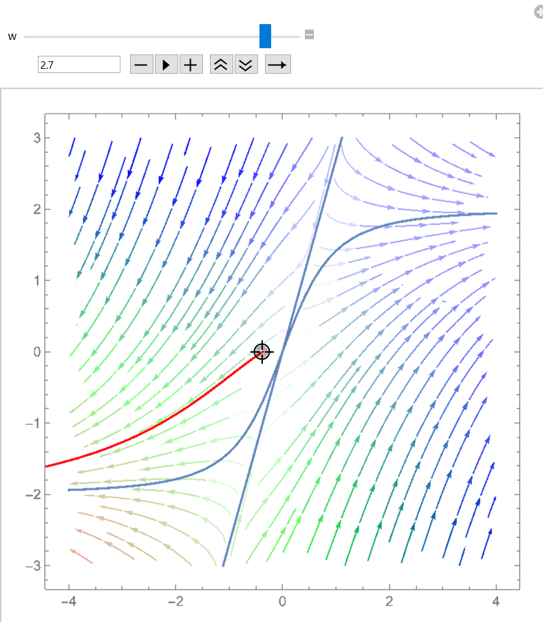
\includegraphics[scale=0.3]{ StabilitySketch01.png}
  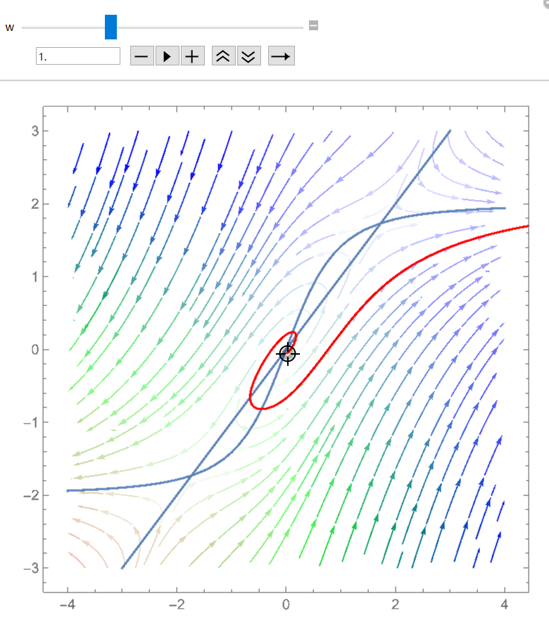
\includegraphics[scale=0.3]{ StabilitySketch02.png}
\\
\footnotesize{Graph 4. The simulation done with Listing 1. at $w=0.1,2.7$, and $1$ respectively.}
\end{center}

Since the state of stability is already discussed, we now focus on under which condition the limit cycle will appear. First, we consider the Poincaré' Index Theorem, which states:
\begin{theorem}[Poincaré Index Theorem]
Any closed orbit in the phase plane must enclose equilibria whose indices sum to $+1$. Either a node or a focus have index $+1$. A saddle point has index $-1$.
\end{theorem}

Accordingly, in all cases we discussed above, the limit cycle exist only when $\gamma>1$ ($\Delta>1$, in which case the fixed point $(0,0)$ is not a saddle), and it cannot enclose other two equilibria. Moreover, in this case, for an asymptotically stable limit cycle to exist, the fixed point enclosed in the limit cycle must be an unstable spiral or node. Therefore, an asymptotically stable limit cycle exists only when $w>d$ and $\gamma>1$.

Second, we consider the Bendixson's Theorem, which states:
\begin{theorem}[Bendixson's Theorem ]
  For a planar system $\mathbf{x'=f(x)}$ defined in a simply connected domain $D\in \mathbb{R}^2$. Assume that $f_1,f_2$ have continuous partial derivatives in $D$, and that $\mathbf{div} \mathbf{f=\nabla f}=\frac{\partial f}{\partial x}+\frac{\partial g}{\partial y}$ does not change sign in $D$. Then the system $\mathbf{x'=f(x)}$ does not have any non-constant periodic orbits in $D$.
\end{theorem}
  Conversely, for a limit cycle to exist, it must cross the line  $\frac{\partial f}{\partial x}+\frac{\partial g}{\partial y}=0$. In this particular case, $\frac{\partial f}{\partial x}+\frac{\partial g}{\partial y}=0$ gives two lines (symmetric about the origin and parallel with each other):

  \begin{equation}
    wx-by\pm \frac{1}{b}\sqrt{\frac{w}{d}^{\frac{3}{2}]}-1}=0
  \end{equation}

  Given the discussion above, a ring shaped region centered at the origin will have the maximum radius $r_{max}$ equals to the distance between the origin and a closest equilibrium, and the minimum of its radius $r_{min}$ equals to the distance between the origin and any one of the two lines. In this case, they are given by:

\begin{equation}
  \begin{matrix}
    r_{min}=\frac{w\sqrt{(\frac{w}{d})^{\frac{3}{2}}-1}}{\sqrt{w^2b^2+1}}\\
    \\
    r_{max}=\sqrt{\frac{(\gamma^2-1)}{c^2}(1+\frac{w^2}{b^2})}
  \end{matrix}
\end{equation}

\begin{center}
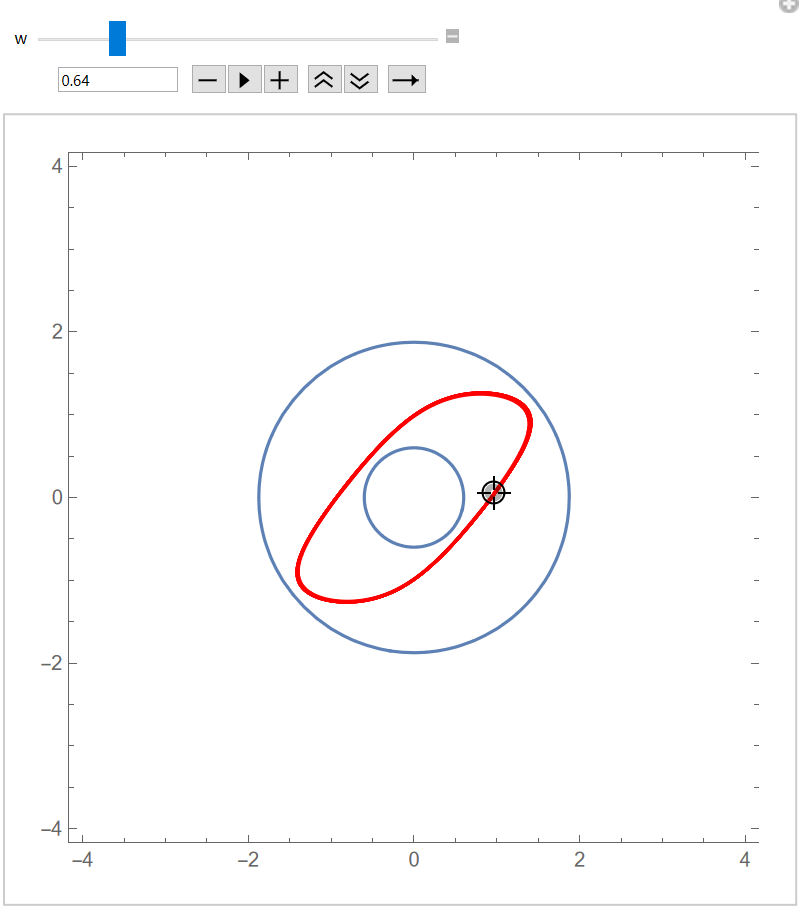
\includegraphics[scale=0.38]{ RminRmax01.png}\\
\footnotesize{Graph 5. The ring shaped region and the limit cycle at $b=1,c=1,d=0.5,w=0.67$.}
\end{center}

Since the shape of the limit cycle in this model is not  necessarily a circle centered at $(0,0)$, the ring-shaped region is not strictly the region that the limit cycle must stay in, but provides a rough region that the limit cycle may exist in. Meanwhile, $r_{min}$ and $r_{max}$ must be real values, which gives the range that $w>d$ and $\gamma>1$, which coincides with the range of $w$ and $\gamma$ in our previous analyses.

After obtaining this range with theoretical analysis, we then use numerical analysis to see how the existence of an asymptotically stable limit cycle changes as $w$ changes. Following the previous example, we again take $b=1,c=1,d=0.5$ and change $w$ to check the existence of an asymptotically stable limit cycle. We use Mathematica to draw the phase portraits for different value of $w$ (code in Listing 1), and obtained the results in Graph 6.

\begin{center}
  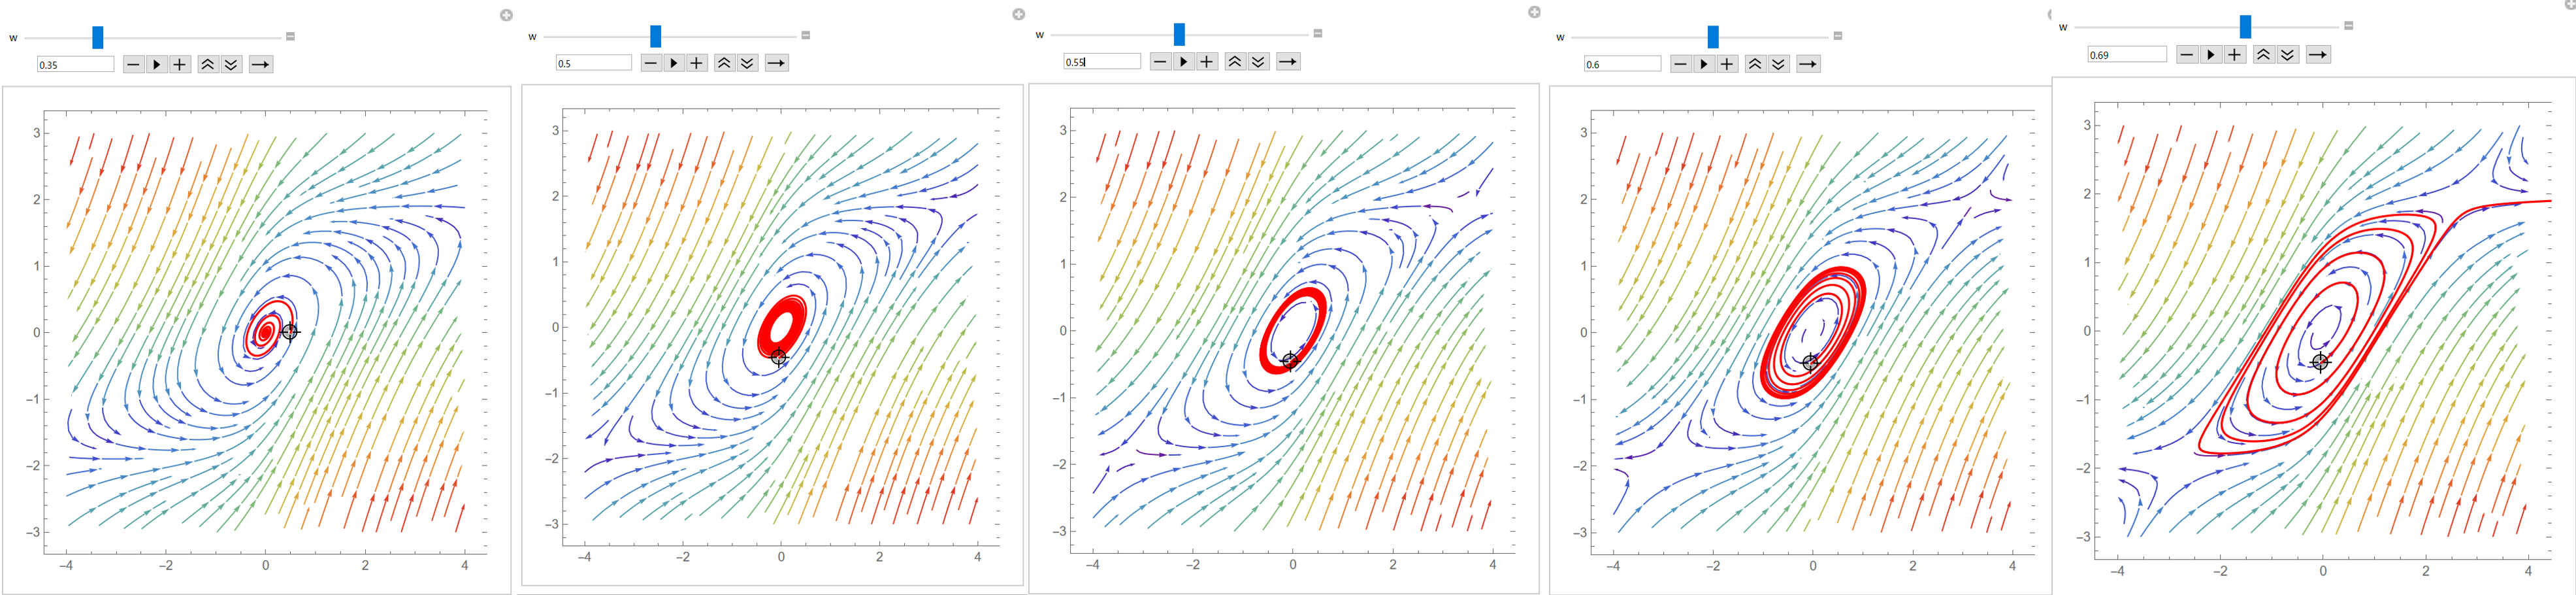
\includegraphics[scale=0.5]{ LimitCycleExplanation.png}\\
  \footnotesize{Graph 6. The solution trajectories at $w=0.35,0.5,0.55,0.6,0.69$.}
  \end{center}

  We observe that the limit cycle appears $w=0.5$, which agrees with our theoretical analysis. At $w=0.5$, $T$ changes from negative to positive and the Hopf Bifurcation takes place. As $w$ grows, the size of limit cycle grows and finally reach $r_{max}$, where it disappears.

  This process can be quantitatively illustrated by the relationship between the period of the limit cycle and $w$. The period-$w$ relationship obtained by Monteiro. et. al(2002) is shown in Graph 7. 

  \begin{center}
    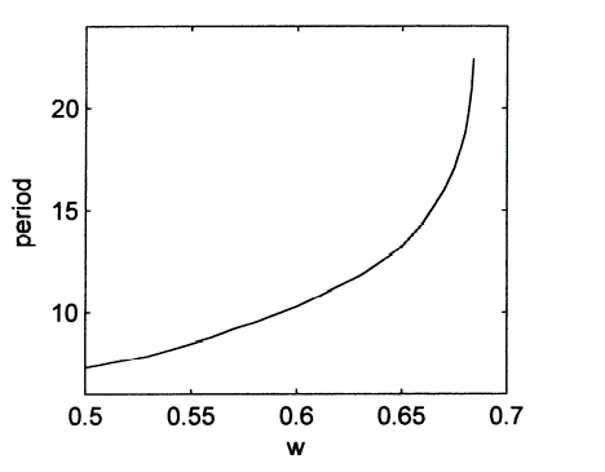
\includegraphics[scale=0.5]{ PeriodExplanation.png}\\
    \footnotesize{Graph 7.The period-$w$ relationship at b=1,c=1,d=0.5, Monteiro.et. al (2002, p. 87).}
    \end{center}

In Graph 7, we can observe that the limit cycle appears at $w=0.5$. As $w$ increases, the period keeps increasing and when $w\to 0.7$, period$\to\infty$, which agrees with our previous observation.

In the particular case, when $a = 0, b = 1, c = 1, d = 0.5, w=0.6$, we also use python to simulate the system and the activities of excitatory and inhibitory cells (code in Listing 2). In Graph 8, we can see that the solution start from the point $(2,2)$ would approach the limit cycle as t increases, which corresponds to our previous assumption. If we record each $x, y$ coordinates as a function of t, then it would give rise to the two curves shown in the Graph 9. The blue curve represents the excitatory cells while the orange curve represents inhibitory cells. As t increases, the two curves become periodic which represents the oscillatory behavior of the cells. 
We also want to see how does the periods of the limit cycles change as the variable w changes. To calculate the period for each $w_0$, we find the time intervals between each local maximum and when the difference of the time interval is less than the threshold (set as $0.2$), we decide to make the time interval as the period at $w_0$. In this simulation, we take 100 different values for w and make the period-w curve in the Graph 10. The result also fits our assumption.

\begin{center}
  \includegraphics[scale=0.3]{ Py-simu-01.jpg}\\
  \footnotesize{Graph 8.The dynamics of the system at $a=0,b=1,c=1,d=0.5,w=0.6$.}
  \end{center}

\begin{center}
  \includegraphics[scale=0.5]{ Py-simu-03.png}\\
    \footnotesize{Graph 9.The behavior of $x,y$ at $a=0,b=1,c=1,d=0.5,w=0.6$.}
  \end{center}

  \begin{center}
    \includegraphics[scale=0.5]{ Py-simu-02.png}\\
      \footnotesize{Graph 10.The period of the system at $a=0,b=1,c=1,d=0.5,w=0.6$.}
    \end{center}


\subsection{Other Cases}

We also study other cases that can influence the occurrence of a limit cycle. The general case is too complex to be study and we find it necessary to pin down other parameters to analysis the model. Here we specifically focus on the change of external simulations ($I,J$) and its influence on the occurrence of a limit cycle.

\subsubsection{$J=0$, Pin down other parameters and change $I$}

The first case we study is $J=0$ and the changes in the state of a limit cycle as $I$ changes. Through simulation in Mathematica we find the results in Graph 11 (with code in Listing 3). 

\begin{center}
  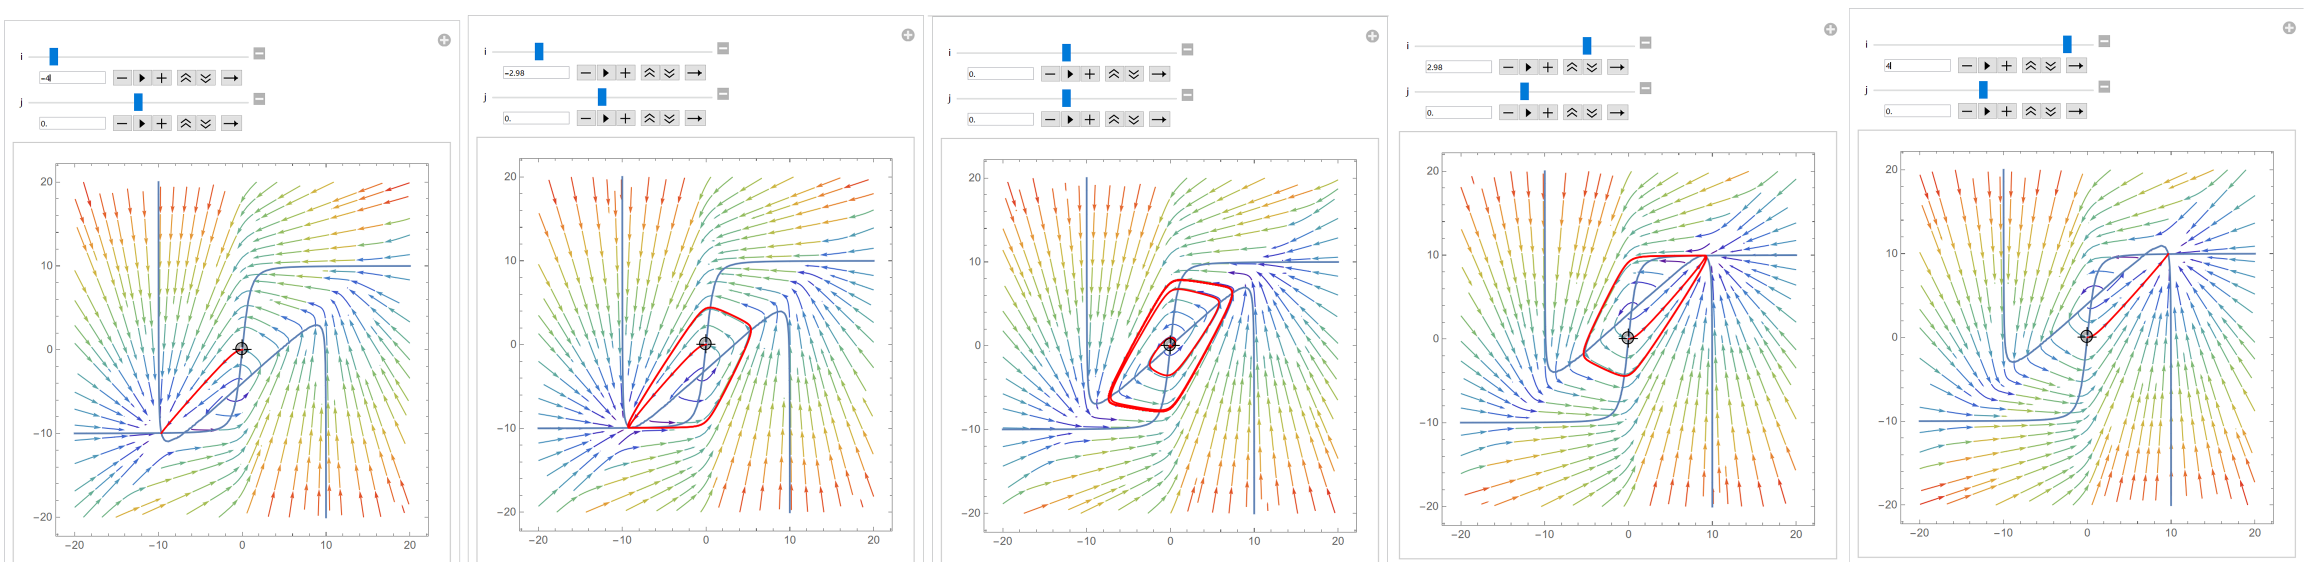
\includegraphics[scale=0.4]{ I-exp.png}\\
  \footnotesize{Graph 11. The solution trajectories at $I=-4,-2.98,0,2.98$ and $4$.}
  \end{center}

We observe that the nullcline $y_f(x)$ moves up vertically as $I$ increases. The limit cycle exists when $I\in [-2.98,2.98]$. In this range $y_f(x)$ and $y_g(x)$ has only one intersection $x_0^*$ between $x_1$ and $x_2$, and $x_0^*$ is always unstable. One explanation for this is the limit cycle moves as $x_0^*$ moves and it get closer to other equilibrium and its period gets larger. As the nullclines get closer to the intersection point, the period of the limit cycle tends to infinity and the limit cycle disappears when it reaches other equilibrium. The period-$I$ relationship found by Monteireo et. al.(2002) is shown in Graph 12, and the result agrees with this explanation.

\begin{center}
  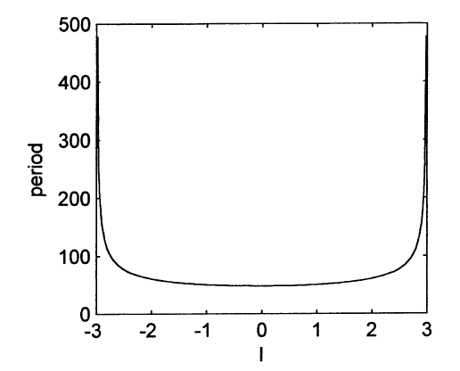
\includegraphics[scale=0.7]{GeneralCase01_1.png}\\
  \footnotesize{Graph 12. Period-$I$ relationship found by Monteireo et. al (2002,p. 89)}
  \end{center}


\subsubsection{$I=0$, Pin down other parameters and change $J$}

The second case we study is $I=0$, and the changes in the state of a limit cycle as $J$ changes. Similarly, with simulation in Mathematica we get result in Graph 12 (with code in Listing 3).

\begin{center}
  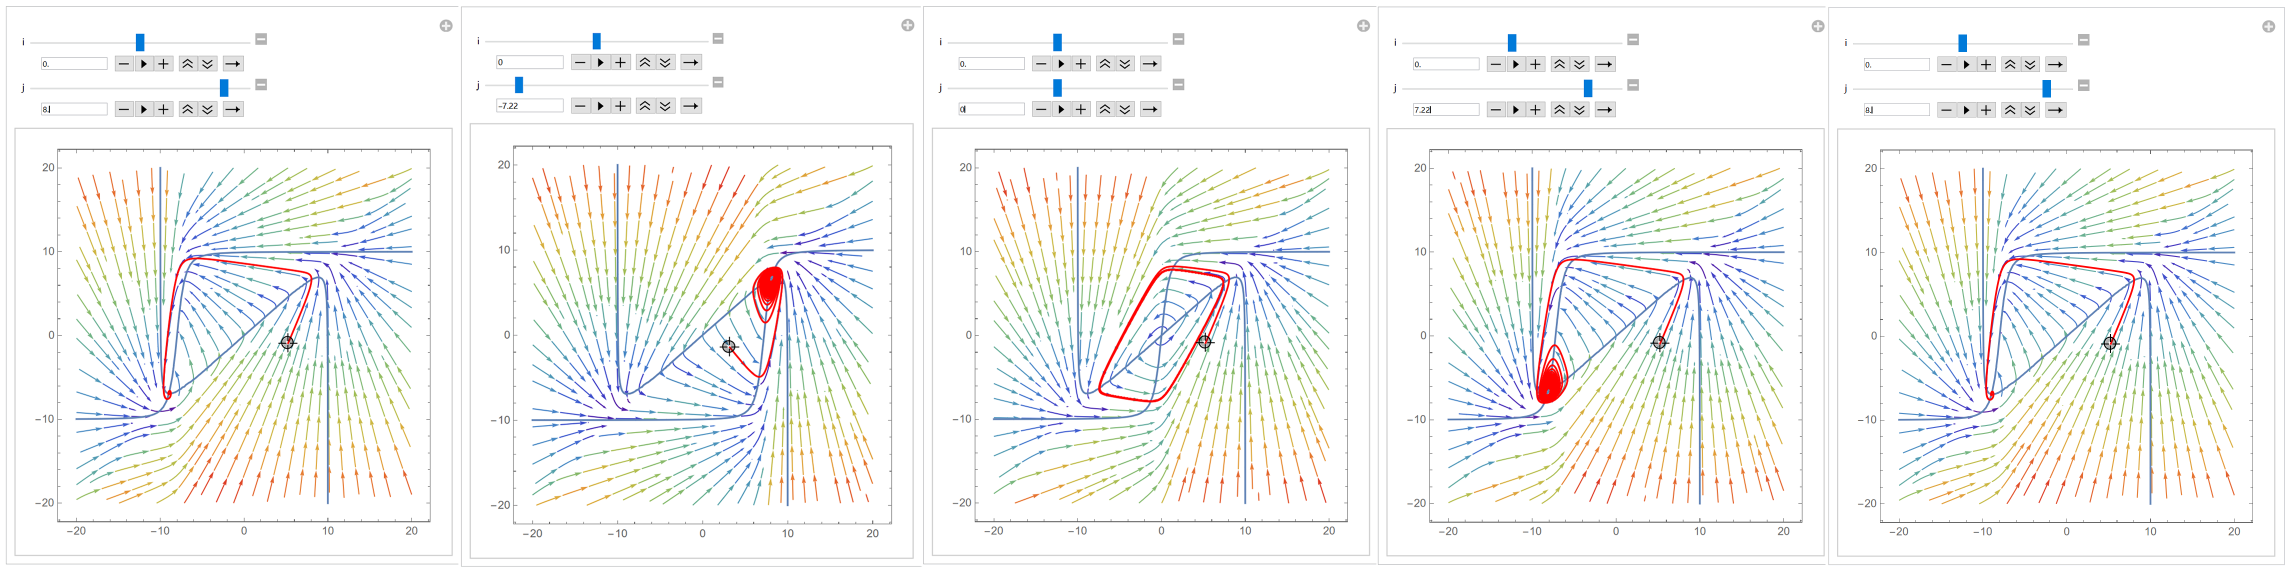
\includegraphics[scale=0.4]{ J-exp.png}\\
  \footnotesize{Graph 13. The solution trajectories at $I=-8,-7.22,0,7.22$ and $8$.}
  \end{center}

We observe that the nullcline $y_g(x)$ moves left horizontally as $J$ increases. The limit cycle exists when $I\in [-7.22,7.22]$. In the whole process the nullcline $y_f(x)$ and $y_g(x)$ always has and only has one intersection, while the stability of this equilibrium change from stable to unstable and then to stable as J increases. The bifurcation happens when $J=7.22$ and $J=-7.22$, where $T$ is close to $0$ ($T=\pm 0.002$) and $\Delta>0$. The limit cycle gets smaller and same as the period of the limit cycle as the $J$ get closer to the point where the system goes through Hopf Bifurcation and disappears when the equilibrium changes from unstable to stable. The period-$J$ relationship found by Momteireo et. al is shown in Graph 13 and the result agrees with this explanation. 

\begin{center}
  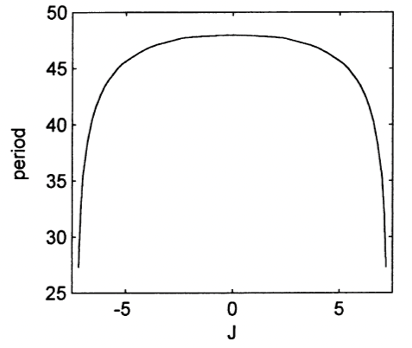
\includegraphics[scale=0.7]{GeneralCase02_1.png}\\
  \footnotesize{Graph 14. Period-$J$ relationship found by Monteireo et. al. (2002, p. 90). }
  \end{center}
  
\subsubsection{Another finding}

Another finding of this model is when $w=0$, $T=-a-d$。 In this case $T$ is constantly negative and the equilibria of the system can only be saddle or stable, and a limit cycle cannot exist. Therefore, we conclude that $w>0$ is a key to the occurrence of a limit cycle. In other words, the self-excitatory factor is necessary for the oscillatory behavior. 

\section{ Conclusion and Discussion} 

In our project, we try to answer the question that under which conditions the oscillatory behavior of the neural response may appear. In the particular case (I=0, J=0), we make the external stimulations as zero and explore the dynamics of the system as w changes. We found that when we take $a=0,b=1,c=d,d=0.5$, the limit cycle in the planar system would appear when w belongs to a rough range (0.5, 0.7). And the period of the limit cycle increases as w increases. The particular case showed that even an unstimulated cortical column can oscillate. Thus, the oscillations behavior may be explained as an intrinsic characteristic of dynamical competition between excitatory and inhibitory neurons. 

We also found that the oscillatory behavior and such a behavior only occur when $w>0$ (self-excitatory connections exist), then the presence of self-excitatory connection may be important for the oscillation. 

In other cases, since there are too many cases, we only do two attempts. When we change the external stimulation to the system, we observe that when we set $I=0$ and change $J$, the Hopf Bifurcation takes place and accordingly the limit cycle appears and disappears (the limit exists when $J\in [-7.22,7.22]$); when we set $J=0$ and changes $I$, we observe the position of limit cycle changes and it disappears when enclosing other equilibrium (the limit cycle exists when $I \in [-2.98,2.98]$).

As we change different values of the variables, The model here shows that the period of a limit cycle could also be changed. Therefore, the activity of cortical columns can oscillate in different natural frequencies. Our results also suggest a partial solution to the  problem.

Further explorations can be done by researching the influences of changes in other parameters have on the occurrence of a limit cycle and discuss their practical significance. 

\section{ Appendix}

\begin{lstlisting}[language=Mathematica, caption=Wilson-Cowan Simulation-Mathematica]
  i=0
  j=0
  a=0
  b=1
  c=1
  d=0.5
  Manipulate[
  Show[ StreamPlot[{-a x + (w x - b y + i)/
    Sqrt[(w x - b y + i)^2 + 1], -d y + (c x + j)/
    Sqrt[(c x + j)^2 + 1]}, {x, -4, 4}, {y, -3, 3}, 
 StreamColorFunction -> (Opacity[#5, 
     Blend[{Red, Green, Blue}, Norm[{#1, #2}]]] &)], 
ContourPlot[-d y + (c x + j)/Sqrt[(c x + j)^2 + 1] == 0, {x, -4, 
  4}, {y, -3, 3}, ColorFunction -> Yellow], 
ContourPlot[-a x + (w x - b y + i)/Sqrt[(w x - b y + i)^2 + 1] == 
  0, {x, -4, 4}, {y, -3, 3}, ColorFunction -> Yellow], 
ParametricPlot[Evaluate[First[{x[t], y[t]} /.
    NDSolve[{x'[
        t] == -a x + (w x[t] - b y[t] + i)/
         Sqrt[(w x[t] - b y[t] + i)^2 + 1], 
      y'[t] == -d y[t] + (c x[t] + j)/Sqrt[(c x[t] + j)^2 + 1], 
      Thread[{x[0], y[0]} == point]}, {x, y}, {t, 0, 100}]]], {t, 0,
   100}, PlotStyle -> Red]], {{point, {0.5, 0}}, Locator}, {w, 0.1, 
3}, SaveDefinitions -> True]
  \end{lstlisting}


\begin{lstlisting}[language=Python, caption=Wilson-Cowan Simulation-Python-Run in an IPython Notebook]
# for fast array manipulation
import numpy as np
import math
# for plotting
import matplotlib.pyplot as plt
# for numerical ODE integration
from scipy.integrate import odeint
# for nonlinear equations
from scipy.optimize import fsolve
# to display plots in-line
%matplotlib inline


def cal_period(w):
    def S(x):
        return x / (np.sqrt(np.power(x,2)+1))
    def WilsonCowan(y, t):
        E = y[0]
        I = y[1]
        a = 0
        b = 1
        c = 1
        d = 0.5
        var_1 = 0
        var_2 = 0

        x_gradient = (w * E - b * I + var_1) / np.sqrt(np.power(w * E - b * I + var_1, 2) + 1)
        y_gradient = -d * I + (c * E + var_2) / np.sqrt(np.power(c * E + var_2, 2) + 1)
        return [x_gradient, y_gradient]

    # minimum and maximum x and y values we want displayed in the graph
    minval = -3
    maxval = 3
    resolution = 50
    # State variables
    x1 = np.linspace(minval, maxval, resolution)
    x2 = np.linspace(minval, maxval, resolution)
    # Create a grid for evaluation of the vector field
    x1, x2 = np.meshgrid(x1, x2)
    # Evaluate the slopes
    X1, X2 = WilsonCowan([x1, x2], 0)
    # Compute the magnitude vector
    M = np.hypot(X1, X2)
    
    fixed_p = []
    y1 = x1.ravel()
    y2 = x2.ravel()
    for i in range(resolution**2):
        # find a zero
        sol, infodict, ier, mesg = fsolve(WilsonCowan, [y1[i], y2[i]], args=(0), full_output=1)
        if ier == 1: 
            fixed_p.append(sol)

    fixed_p = np.array(fixed_p).T
    time = np.linspace(0, 100, 2000)
    E0, I0 = 2, 2 
    # find the solution with scint.odeint
    odesol = odeint(WilsonCowan, [E0, I0], time)
    # separate the two solutions
    exc_timeseries, inh_timeseries = odesol.T
    
    for i in range(1, len(exc_timeseries) - 1):
        if exc_timeseries[i] <= exc_timeseries[i - 1] and exc_timeseries[i] <= exc_timeseries[i + 1]:
            temp_start = i
            for j in range(i + 1, len(exc_timeseries) - 1):
                if exc_timeseries[j] <= exc_timeseries[j - 1] and exc_timeseries[j] <= exc_timeseries[j + 1]:
                    temp_end = j
                    if abs(exc_timeseries[temp_end] - exc_timeseries[temp_start]) < 0.2:
                        start = temp_start
                        end = temp_end
                        break
                    else:
                        temp_start = temp_end
            break
    return end - start

w_test = np.linspace(0.5, 0.675, 100)
period_array = []
for i in w_test:
    period_array.append(0.05 * cal_period(i)) 
    print(cal_period(i))
    
plt.plot(w_test, period_array)
plt.ylabel(r'$period$')
plt.xlabel(r'$w$')

# plotting the vector field
plt.figure(figsize=(10, 10))
plt.quiver(x2, x1, X2, X1, pivot='mid', alpha=.5)
plt.xlim([minval, maxval])
plt.ylim([minval, maxval])
plt.xlabel(r'$y$', fontsize=16) # yes, you can use Latex code!
plt.ylabel(r'$x$', fontsize=16)
plt.grid()

# plot the solution in the state space
plt.plot(inh_timeseries, exc_timeseries, '.-');

# plot the starting point
plt.scatter(I0, E0, marker='*', s=300, label="Starting point")
plt.legend(loc="upper left")

# plot the equilibria we identified
plt.scatter(fixed_p[1], fixed_p[0], marker='o', s=50, label="Stationary points")

# plot the solution in time
plt.figure(figsize=(10.3,3))
plt.ylabel(r'$x, y$')
plt.xlabel(r'$t$')
plt.plot(time, exc_timeseries, '.-', label="excitatory");
plt.plot(time, inh_timeseries, '.-', label="inhibitory");
plt.legend();
      \end{lstlisting}

\begin{lstlisting}[language=Mathematica, caption=Wilson-Cowan Simulation-Mathematica]
  a = 0.1
  d = 0.1
  b = 1
  c = 1
  w = 1
  Manipulate[
   Show[ StreamPlot[{-a x + ( w x - b y + i)/
        Sqrt[(w x - b y + i)^2 + 1], -d y + (c x + j)/
        Sqrt[(c x + j)^2 + 1]}, {x, -20, 20}, {y, -20, 20}, 
     StreamColorFunction -> "Rainbow"], 
    ContourPlot[-d y + (c x + j)/Sqrt[(c x + j)^2 + 1] == 0, {x, -20, 
      20}, {y, -20, 20}, ColorFunction -> Yellow], 
    ContourPlot[-a x + (w x - b y + i)/Sqrt[(w x - b y + i)^2 + 1] == 
      0, {x, -20, 20}, {y, -20, 20}, ColorFunction -> Yellow], 
    ParametricPlot[Evaluate[First[{x[t], y[t]} /.
        
        NDSolve[{x'[
            t] == -a x[t] + ( w x[t] - b y[t] + i)/
             Sqrt[(w x[t] - b y[t] + i)^2 + 1], 
          y'[t] == -d y[t] + (c x[t] + j)/Sqrt[(c x[t] + j)^2 + 1], 
          Thread[{x[0], y[0]} == point]}, {x, y}, {t, 0, 1000}]]], {t, 
      0, 1000}, PlotStyle -> Red]], {{point, {0.02, 0}}, 
    Locator}, {i, -5, 5}, {j, -10, 10}, SaveDefinitions -> True]
  \end{lstlisting}
  
  
  
\clearpage
      
\phantomsection
\addcontentsline{toc}{section}{References}      
\begin{thebibliography}{9}

  \bibitem{lamport94}
  Ashby, W. R., H. Von Foerster, \& C. C. Walker. 1962. Nature (London). 196:561.
  Griffth, J. S. 1963. Biophys. J. 3:299.
  
  \bibitem{lamport94}
  Basar, E., Basar-Eroglu C., Karakas S. \& Schurmann M. (1999). Oscillatory brain theory: a new trend in neuroscience. IEEE Eng. Med. Biol. 18, 56–66.

  \bibitem{lamport94}
  Engel, A. K., Ko. nig, P. \& Schillen, T. B. (1992b). Why does the cortex oscillate? Curr. Biol. 2, 332–334.

  \bibitem{lamport94}
  H. R. Wilson and J. D. Cowan. “Excitatory and Inhibitory Interactions in Localized Populations of Model Neurons”. In: Biophysical Journal 12.1 (1972), pp. 1–24. doi: 10 . 1016 / S0006 - 3495(72)86068-5
  
    \bibitem{texbook}
  L. H. A. Monteiro, M. A. Bussab, and J. G. Chaui Berlinck, “Analytical results on a Wilson-Cowan neuronal network modified model,” Journal of Theoretical Biology, vol. 219, no. 1, pp. 83–91, 2002.

  
  \bibitem{lamport94}
  Von der Malsburg C. \& Buhmann, J. (1992). Sensory segmentation with coupled neural oscillators. Biol. Cybern. 67, 233–242.
\end{thebibliography}

\end{document}


